\label{app:protocolo}

\subsection*{Entrevista a usuario final}

\begin{enumerate}
    \item ¿En qué tareas del hogar le gustaría que un robot lo asista?
    \item ¿Hay actividades que preferiría hacer usted mismo en lugar de delegarlas a un robot? ¿Por qué?
    \item ¿Qué tanto espera que el robot trabaje de forma autónoma en lugar de recibir órdenes explícitas?
    \item ¿Cuánto tiempo cree que debería tomarle a un robot realizar sus tareas respecto al tiempo que le tomaría a una persona?
    \item Si usted saliera de viaje y el robot se quedara solo en su casa, ¿qué le pediría que hiciera en su ausencia?
    \item ¿De qué manera le gustaría poder dar órdenes al robot (escritas, habladas, desde un control, una computadora)?
    \item ¿De qué forma se imagina que sería más fácil confirmar que el robot realmente entendió la órden que está por ejecutar?
    \item ¿Le gustaría que el robot le reportara el estatus de las actividades encargadas? ¿En qué forma le gustaría que lo hiciera?
    \item ¿Qué tan importante le parece que el robot parezca una persona?
    \item ¿Cree que el robot debería cambiar su comportamiento dependiendo de con quién interactúa? En caso afirmativo, ¿de qué forma?
    \item ¿Qué artículo del hogar le daría más miedo permitir que un robot manipule?
    \item ¿Cuáles son los objetos más pesados o frágiles sería útil para usted que el robot pudiera manipular?
    \item Además de objetos y bolsas, ¿qué otro tipo de cosas crees que sería útil que el robot pudiera manipular? Ej. Puertas, llaves, cepillos
    \item ¿Le gustaría que el robot incluyera un manual para que usted mismo le pudiera dar mantenimiento y hacer reparaciones básicas o preferiría llevarlo con el proveedor directamente ante cualquier falla?
    \item ¿Utilizaría el robot únicamente en su hogar o consideraría llevarlo consigo para que lo asista en viajes?
    \item ¿La apariencia de qué robot le inspira mayor confianza? ¿Por qué?
    
    \begin{figure}[h]
        \centering
        \begin{subfigure}{0.3\linewidth}
            \centering
            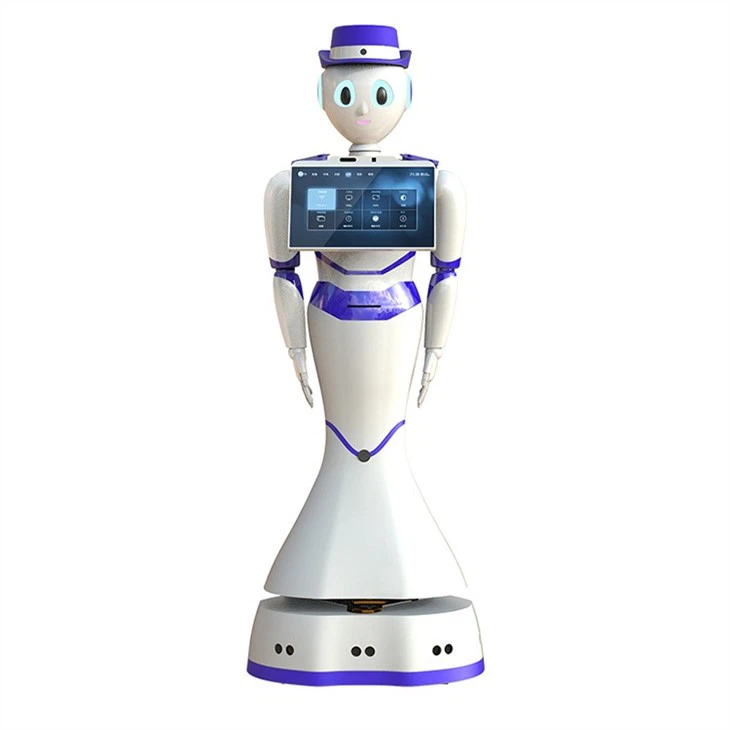
\includegraphics[width=\linewidth]{img/appendix/reeman5.png}
            \caption{Opción 1}
            \label{fig:image1}
        \end{subfigure}
        \hfill
        \begin{subfigure}{0.3\linewidth}
            \centering
            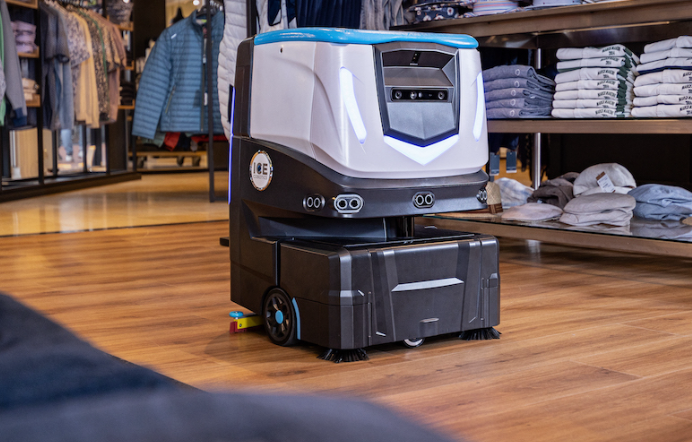
\includegraphics[width=\linewidth]{img/appendix/ice_cobotics.png}
            \caption{Opción 2}
            \label{fig:image2}
        \end{subfigure}
        \hfill
        \begin{subfigure}{0.3\linewidth}
            \centering
            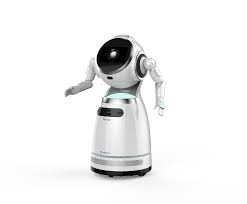
\includegraphics[width=\linewidth]{img/appendix/cruzr.jpeg}
            \caption{Opción 3}
            \label{fig:image3}
        \end{subfigure}        
    \end{figure}
    
    \item ¿Cuáles son las principales preocupaciones que le generaría tener un robot de servicio en casa?
    \item ¿Qué elementos podría incluir el robot para hacerlo sentir más seguro?
\end{enumerate}

\subsection*{Entrevista al desarrollador de software (General)}

\begin{enumerate}
    \item Cuéntanos acerca de tu experiencia en la RoboCup, enfocada principalmente a la categoría @Home.
    \item ¿Cuáles han sido los problemas más importantes que has enfrentado o te has enterado que han enfrentado otros equipos durante una competencia?
    \item ¿Cuál consideras que es el hardware mínimo que se requiere para participar en esta categoría? ¿Cuál de  esos elementos consideras que tiene un mayor impacto en el desempeño del robot?
    \item ¿Consideras que la apariencia del robot afecta la manera en la que el usuario interactúa con él? ¿Crees que este efecto tiene un impacto real en su desempeño?
    \item Además de las instrucciones que se le dan a un usuario no experto antes de una prueba, ¿qué otros elementos integrados en el robot has notado que hacen más intuitiva la interacción?
    \item ¿Qué otras formas de interacción se han usado cuando el usuario no domina el idioma inglés?
    \item ¿Has identificado alguna característica del diseño de los manipuladores, que nosotros u otros equipos hayan implementado, que pudiera incomodar/lastimar al usuario?
    \item ¿Qué tareas de manipulación consideras más críticas en la competencia?
    \item ¿Cuál consideras una mejor característica al tomar objetos: la velocidad o la precisión? ¿Por qué?
    \item ¿Cuál has identificado como el principal motivo por el que a un robot se le caen objetos que ya había tomado?
    \item ¿Cuál es el objeto más grande o pesado que se debe tomar en las pruebas?
    \item ¿Cuál es el objeto más pequeño y delicado que se ha tenido que manipular en las pruebas?
    \item ¿Hay alguna otra característica, además del peso y tamaño, que haga complicado tomar un objeto? (Ej. Rugosidad de la superficie)
    \item ¿Qué condiciones de luz has identificado que afectan más a los sistemas de percepción del robot?
    \item ¿Has identificado problemas con puntos ciegos del robot en la competencia?
    \item ¿Consideras que la medición de par o fuerza en las articulaciones del brazo y gripper sería útil?
    \item ¿Qué medidas de redundancia crees que sean más importantes para la seguridad y el rendimiento del robot?
    \item ¿Qué elementos de seguridad, además del botón de paro, consideras que es importante incluir en el diseño del robot?
\end{enumerate}

\subsection*{Entrevista al desarrollador de software (Plataforma experimental)}

\begin{enumerate}
    \item ¿Cuáles consideras que son las características clave del manipulador para tomar objetos y cuáles pueden ser compensadas con la posición de la base?
    \item ¿Cuál recuerdas como el efector final más efectivo en la competencia?
    \item ¿Crees que la integración de una cámara en el gripper mejoraría su habilidad de tomar objetos?
    \item ¿Hay alguna característica del robot que consideres importante como el peso o el tamaño? Más allá de las limitaciones que impone el reglamento.
    \item En caso de contar con un robot de dos brazos, ¿consideras que deberían ser brazos idénticos o cada brazo debería tener una habilidad diferente? ¿El efector final debería ser intercambiable?
    \item En los diseños previos, ¿qué partes del hardware eran más inaccesibles para su mantenimiento?
\end{enumerate}

\subsection*{Entrevista al desarrollador de software (Plataforma comercial)}

\begin{enumerate}
    \item ¿Cuáles consideras que son las mayores virtudes del hardware de Takeshi?
    \item Si pudieras modificar algo, ¿lo harías? ¿qué sería?
    \item ¿Crees que la integración de la cámara en el gripper mejora su habilidad de tomar objetos o sólo incrementa el tiempo de procesamiento? ¿Sí la utilizan?
    \item ¿Considerarías útil que el efector final fuera intercambiable?
    \item ¿Qué tareas de manipulación consideras que son las más desafiantes considerando que Takeshi solo cuenta con un brazo?
    \item ¿Han tenido que compensar las limitaciones de los grados de libertad que proporciona Takeshi? ¿Cómo lo han hecho?
    \item ¿Han tenido que compensar las limitaciones de los grados de libertad que proporciona Takeshi? ¿Cómo lo han hecho?
    \item ¿Existe alguna limitación en el mantenimiento del hardware considerando que se trata de un robot comercial?
    \item Dado que todos tienen el mismo hardware, ¿qué utilizas como diferenciador?
\end{enumerate}

\section*{Riesgos y beneficios anticipados}

\subsection*{Riesgos}
Esta investigación presenta riesgos mínimos para los participantes. No se utiliza instrumento alguno o contacto con el robot de ningún tipo y únicamente involucra preguntas sobre experiencias técnicas y necesidades cotidianas.

Los riesgos identificados incluyen:

\begin{itemize}
\item Posible incomodidad al compartir información sobre necesidades personales de asistencia doméstica.
\item Fatiga durante la sesión de entrevista (mitigado mediante sesiones de duración razonable con pausas si es necesario).
\item Riesgo mínimo de identificación indirecta a pesar de la codificación de datos.
\end{itemize}

\subsection*{Beneficios}
Los participantes podrán obtener los siguientes beneficios:

\begin{itemize}
\item Contribución directa al desarrollo de tecnología de asistencia robótica que puede mejorar la calidad de vida de personas con necesidades similares.
\item Oportunidad de reflexionar sobre sus experiencias y necesidades, lo cual puede generar aprendizajes valiosos para su propio contexto.
\item Retroalimentación que puede enriquecer su perspectiva sobre el diseño centrado en el usuario.
\item Participación en investigación que busca cerrar la brecha entre el desarrollo tecnológico y las necesidades reales de los usuarios finales.
\end{itemize}

\section*{Criterios de selección}

Los participantes serán seleccionados mediante muestreo intencional conforme a dos perfiles específicos:

\subsection*{Perfil 1: Equipo de desarrollo}
\begin{itemize}
\item Ser miembro activo o previo del equipo de desarrollo del robot de servicio doméstico Justina.
\item Contar con experiencia de participación en la competencia RoboCup@HOME.
\item Tener conocimiento técnico sobre el diseño, programación o implementación de funcionalidades del robot.
\end{itemize}

\subsection*{Perfil 2: Usuarios potenciales}
\begin{itemize}
\item Ser personas que requieren asistencia doméstica constante debido a edad avanzada (65 años o más) o alguna condición de discapacidad que limite su autonomía en actividades cotidianas del hogar.
\item Residir de forma independiente o semi-independiente en un entorno doméstico.
\item Tener capacidad cognitiva para participar en una entrevista y proporcionar consentimiento informado (o contar con representante legal en caso necesario).
\end{itemize}

\section*{Privacidad y confidencialidad}
Los datos personales recolectados durante la investigación serán utilizados exclusivamente con fines académicos. Se garantizará la privacidad de los participantes mediante consentimiento informado, y la confidencialidad de la información será protegida a través de la codificación de datos, almacenamiento seguro y acceso restringido únicamente al equipo investigador.